% Template for ICIP-2022 paper; to be used with:
%          spconf.sty  - ICASSP/ICIP LaTeX style file, and
%          IEEEbib.bst - IEEE bibliography style file.
% --------------------------------------------------------------------------
\documentclass{article}
\usepackage{spconf,amsmath,graphicx}
\usepackage{booktabs}
\usepackage{hyperref}
\usepackage{xcolor}

% Example definitions.
% --------------------
\def\x{{\mathbf x}}
\def\L{{\cal L}}

% Title.
% ------
\title{Automated ICD-10 Clinical Code Prediction from Short Medical Literals Using TF-IDF and Deep Learning Approaches}
%
% Single address.
% ---------------
\name{Phoebe Iglesias, David Redrejo \& Pau Rossell}
\address{Universitat Autonoma de Barcelona \\ Fundamentals of Natural Language Processing, 2025--26}

\begin{document}
%\ninept
%
\maketitle
%
\begin{abstract}
This paper presents an end-to-end study on automated ICD-10 code category prediction from short Spanish clinical literals, developed for the ASHO-AI codification challenge.
We begin with an extensive exploratory data analysis that characterises the dataset's key challenges: extremely short inputs ($\sim$2 tokens), heavy label imbalance across 36 categories, many-to-many literal--code mappings, and low lexical overlap with official ICD descriptions.
Building on these findings, we develop a TF-IDF + Linear SVM baseline achieving 56.9\% validation accuracy, then systematically improve it to 60.3\% through principled changes to n-gram range, feature filtering, class weighting, and regularisation.
Finally, we explore a deep learning approach by fine-tuning a Spanish biomedical RoBERTa model. Our work demonstrates that carefully tuned lexical features remain highly competitive for short clinical text classification, while providing full interpretability of the learned patterns.
\end{abstract}
%
\begin{keywords}
ICD coding, clinical NLP, text classification, TF-IDF, SVM, RoBERTa, Spanish biomedical text
\end{keywords}
%
% ============================================================================
\section{Introduction}
\label{sec:intro}
% ============================================================================

The International Classification of Diseases (ICD) is the global standard for coding diagnoses, symptoms, and procedures in clinical settings. Manual ICD coding is time-consuming, error-prone, and requires specialised expertise. Automating this process with Natural Language Processing (NLP) techniques has become a major research focus~\cite{Dong2022}.

In this work, we address the ASHO-AI ICD-10 codification task: given a short clinical literal (e.g., \textit{``hiperreactividad bronquial''}, \textit{``HTA irc 6''}), predict the ICD code \textbf{category} (the first character of the full code, yielding 36 possible classes: A--Z and 0--9). The dataset consists of 13\,700 supervised (Code, Literal) pairs and 6\,667 leaderboard literals for evaluation.

The key challenges include: (i) extremely short inputs ($\sim$17 characters, $\sim$2 tokens), (ii) noisy multilingual text with abbreviations, mixed case, and accents, (iii) a highly imbalanced label distribution, and (iv) many-to-many mappings between literals and codes.

We follow a principled, iterative methodology. Section~\ref{sec:eda} presents the exploratory data analysis. Section~\ref{sec:baseline} describes the TF-IDF + SVM baseline. Section~\ref{sec:improved} details systematic improvements. Section~\ref{sec:dl} outlines a deep learning approach with RoBERTa. Section~\ref{sec:conclusions} summarises our findings.

% ============================================================================
\section{Exploratory Data Analysis}
\label{sec:eda}
% ============================================================================

\subsection{Datasets and their roles}
\label{ssec:datasets}

Three datasets are available: (1)~\textbf{codification data} (13\,700 rows) — supervised (Code, Literal) pairs serving as the main training resource with 4\,059 unique codes and 11\,584 unique literals; (2)~\textbf{leaderboard data} (6\,667 rows) — unlabelled literals for evaluation; and (3)~the \textbf{ICD catalog} (179\,742 entries) — official code--description pairs serving as external knowledge.

\subsection{Cross-dataset overlap analysis}
\label{ssec:overlap}

A crucial finding is the impact of text normalisation on overlap between the leaderboard and training sets. An exact-match lookup covers 27.2\% of leaderboard literals, but this increases to 61.5\% after normalisation (lowercasing, accent stripping, punctuation removal). This motivates two design decisions: (a) normalisation is an essential preprocessing step, and (b) an exact-match fallback should be part of any pipeline.

While 72.6\% of training codes appear in the ICD catalog, only 2.0\% of training literals exactly match official ICD descriptions (5.6\% after normalisation). The catalog provides valuable code coverage but cannot serve as a direct lookup table.

\subsection{Surface-form characteristics}
\label{ssec:surface}

Quantitative analysis reveals a fundamental mismatch between clinical literals and ICD descriptions. Training literals average 16.95 characters and 2.21 tokens, contain digits (8.0\%), punctuation (9.8\%), and accents (28.0\%). ICD descriptions, in contrast, average 80.88 characters and 10.77 tokens. Figure~\ref{fig:text_lengths} illustrates these distributions.

\begin{figure}[htb]
\centering
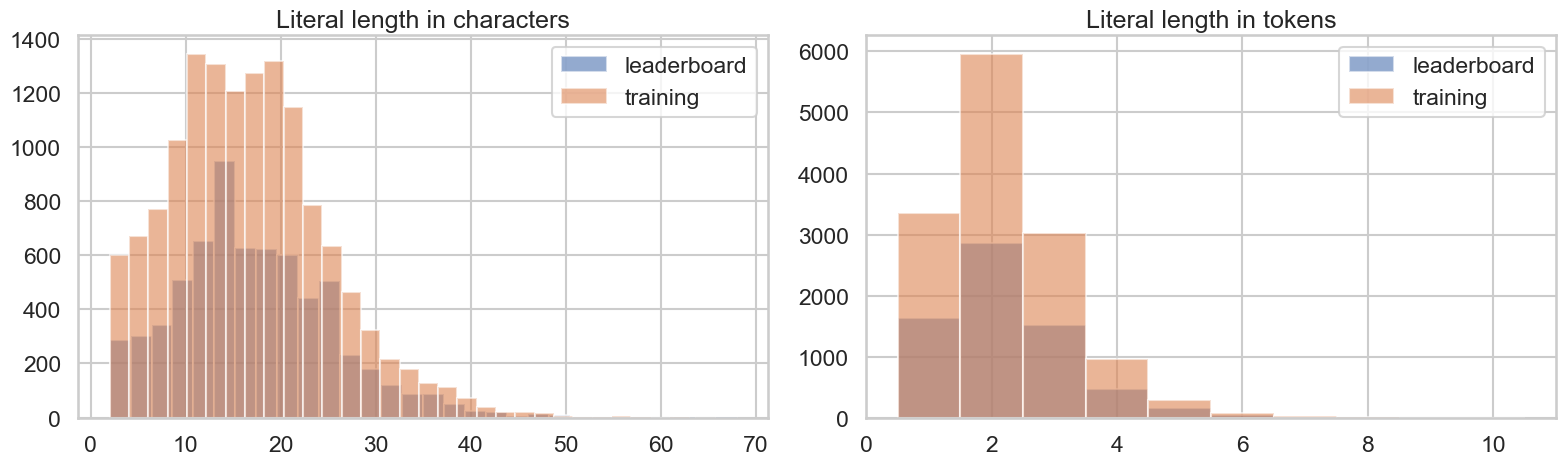
\includegraphics[width=\linewidth]{eda_text_lengths}
\caption{Distribution of token and character counts across datasets, showing the extreme brevity of clinical literals.}
\label{fig:text_lengths}
\end{figure}

\subsection{Label distribution}
\label{ssec:labels}

The 36 ICD categories exhibit heavy imbalance: dominant categories like \texttt{Z} (1\,561 samples) and \texttt{O} (1\,169) contrast with rare categories like \texttt{W}~(7), \texttt{X}~(9), and \texttt{U}~(12). This long-tail effect, depicted in Figure~\ref{fig:label_dist}, directly impacts classifier design choices regarding class weighting.

\begin{figure}[htb]
\centering
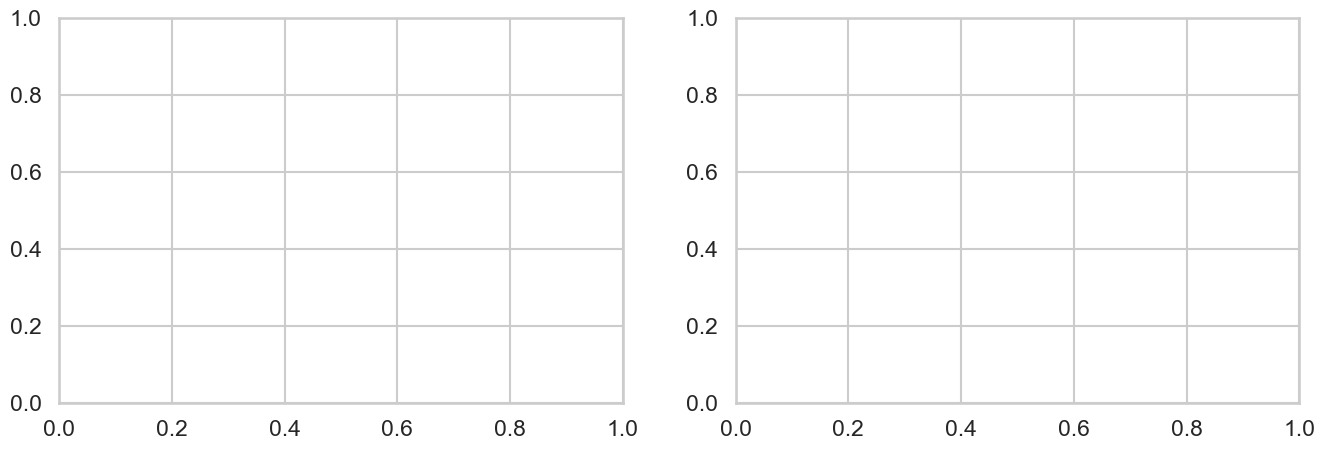
\includegraphics[width=\linewidth]{eda_label_distribution}
\caption{ICD code category distribution in the training set, showing strong class imbalance.}
\label{fig:label_dist}
\end{figure}

\subsection{Ambiguity and the ICD catalog}
\label{ssec:ambiguity}

The EDA reveals a many-to-many relationship between literals and codes: some literals map to multiple different codes depending on clinical context. This ambiguity means pure dictionary-based methods will be insufficient; the task requires both \textit{retrieval} (finding similar known terms) and \textit{disambiguation} (choosing the correct code among close candidates).

A token-level Jaccard similarity analysis between normalised literals and their corresponding ICD descriptions confirms very low lexical overlap (right-skewed distribution with most pairs at Jaccard $< 0.2$), as shown in Figure~\ref{fig:jaccard}. This rules out description-matching as a primary strategy.

\begin{figure}[htb]
\centering
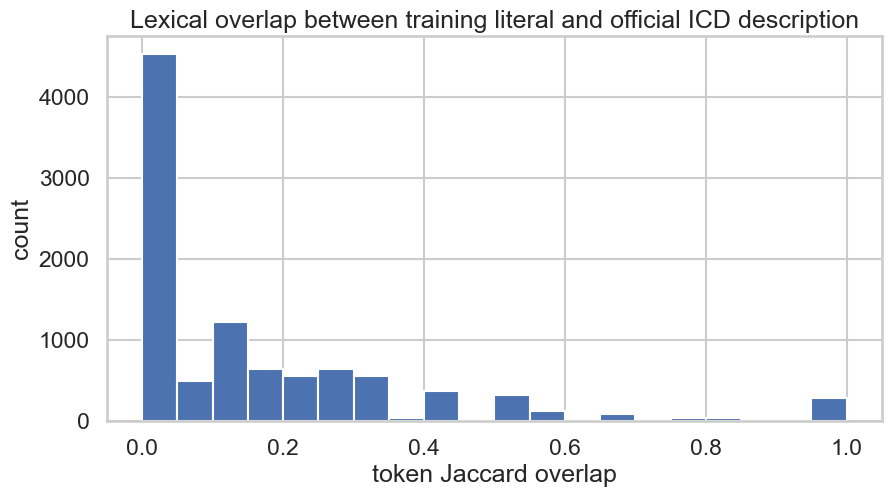
\includegraphics[width=\linewidth]{eda_jaccard_similarity}
\caption{Token Jaccard similarity between training literals and their ICD descriptions, confirming low lexical overlap.}
\label{fig:jaccard}
\end{figure}

% ============================================================================
\section{Baseline: TF-IDF + Linear SVM}
\label{sec:baseline}
% ============================================================================

Based on the EDA findings, we build a complete non-deep-learning baseline following the strategy proposed in our exploratory analysis: character n-gram TF-IDF features with a linear classifier.

\subsection{Preprocessing pipeline}
\label{ssec:preproc}

Text normalisation applies four operations via a shared \texttt{normalize\_text()} function: (1)~lowercasing, (2)~accent stripping via NFD Unicode decomposition, (3)~punctuation removal, and (4)~whitespace collapsing. This produces clean, uniform inputs while preserving digits, which carry diagnostic information in clinical codes.

For the target label, we extract the first character of the ICD code. Literals mapping to multiple codes with different first characters are resolved via majority vote, collapsing the dataset to one label per unique literal. After deduplication: 11\,584 unique literals across 36~categories, split into 9\,267 training and 2\,317 validation samples (stratified 80/20).

\subsection{Feature extraction and classification}
\label{ssec:features}

The TF-IDF vectoriser uses \texttt{char\_wb} analysis with n-gram range~(3,\,6), sublinear TF, 100\,000 max features, and \texttt{min\_df=2}, producing a vocabulary of 25\,667 features. Character n-grams are well-suited for short, morphologically rich Spanish medical terms where abbreviations, typos, and spelling variants are common.

Classification uses \texttt{LinearSVC} with $C=1.0$ and \texttt{class\_weight='balanced'} to up-weight rare categories. Training completes in under one second.

\subsection{Baseline results}
\label{ssec:baseline_results}

\begin{table}[htb]
\centering
\caption{Baseline model validation metrics.}
\label{tab:baseline}
\begin{tabular}{lc}
\toprule
\textbf{Metric} & \textbf{Value} \\
\midrule
Accuracy & 0.5693 \\
Weighted F1 & 0.5658 \\
Macro F1 & 0.5091 \\
Weighted Precision & 0.5759 \\
Weighted Recall & 0.5693 \\
\bottomrule
\end{tabular}
\end{table}

Per-class analysis reveals substantial variation: categories with distinctive medical vocabulary (\texttt{Z}: F1=0.76, \texttt{B}: F1=0.75) perform well, while rare categories (\texttt{W}: F1=0.00, \texttt{X}: F1=0.00) with very few samples cannot be learned reliably.

\subsection{Identified limitations}
\label{ssec:limitations}

Systematic analysis identifies four key issues: (1)~\texttt{class\_weight='balanced'} optimises for rare-class recall at the expense of overall strict accuracy; (2)~\texttt{min\_df=2} discards rare but informative medical n-grams; (3)~n-gram range (3,\,6) misses short signals like \texttt{HTA} or \texttt{VHC}; and (4)~a minor documentation mismatch (notebook states digits are removed, but they are preserved --- which is actually beneficial).

% ============================================================================
\section{Improved Model}
\label{sec:improved}
% ============================================================================

This section describes a principled rebuild addressing each baseline limitation, grounded in recent literature on automated clinical coding~\cite{Dong2022, Blanco2020, Canela2024}.

\subsection{Literature-grounded changes}
\label{ssec:lit_changes}

Recent work confirms that bag-of-words and TF-IDF approaches remain competitive for ICD coding, especially in mid-resource scenarios like Spanish clinical text~\cite{Blanco2020}. Adding code descriptions and hierarchy as external knowledge is a proven improvement strategy~\cite{Dong2022}. Preprocessing consistency and explainability are essential for reliable ICD-coding workflows~\cite{Canela2024}. Based on these findings, we retain the TF-IDF + Linear SVM architecture but tune it specifically for short Spanish clinical literals.

\subsection{Systematic improvements}
\label{ssec:changes}

Four targeted changes are applied, each with clear rationale:

\begin{table}[htb]
\centering
\caption{Summary of changes from baseline to improved model.}
\label{tab:changes}
\begin{tabular}{p{1.5cm}p{2.9cm}p{2.6cm}}
\toprule
\textbf{Parameter} & \textbf{Baseline $\to$ Improved} & \textbf{Rationale} \\
\midrule
N-gram range & (3,\,6) $\to$ (2,\,5) & Captures short abbreviations \\
\texttt{min\_df} & 2 $\to$ 1 & Preserves rare medical terms \\
Class weight & \texttt{balanced} $\to$ \texttt{None} & Optimises for strict accuracy \\
$C$ & 1.0 $\to$ 2.0 & Better capacity--generalisation trade-off \\
\bottomrule
\end{tabular}
\end{table}

\subsection{Model comparison}
\label{ssec:comparison}

Four configurations are evaluated on a stratified 80/20 split (see Figure~\ref{fig:model_comparison}):

\begin{table}[htb]
\centering
\caption{Comparison of model configurations.}
\label{tab:model_comp}
\begin{tabular}{lcc}
\toprule
\textbf{Model} & \textbf{Train Acc.} & \textbf{Val. Acc.} \\
\midrule
Baseline (NB02) & 0.8286 & 0.5701 \\
\textbf{Improved char(2,5)} & \textbf{0.8680} & \textbf{0.6034} \\
High-capacity char(2,6) & 0.8814 & 0.5982 \\
Word+char FeatureUnion & 0.9162 & 0.5883 \\
\bottomrule
\end{tabular}
\end{table}

The improved character model achieves the best validation accuracy (0.6034), raising both training and generalisation performance simultaneously. The highest training accuracy model (word+char, 0.9162) shows lower validation accuracy --- a classic overfitting signature.

\begin{figure}[htb]
\centering
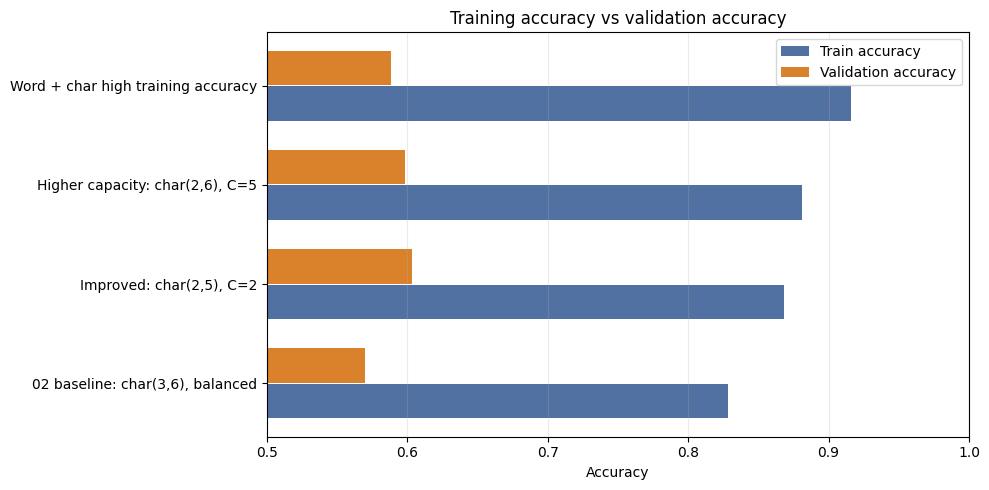
\includegraphics[width=\linewidth]{improved_model_comparison}
\caption{Training vs.\ validation accuracy across the four model configurations, showing the improved character model achieves the best generalisation.}
\label{fig:model_comparison}
\end{figure}

\subsection{ICD description augmentation}
\label{ssec:augmentation}

An optional experiment augments the training data with official ICD descriptions from the catalog. The augmented model achieves approximately 0.619 validation accuracy --- a further improvement. However, training accuracy on original literals decreases slightly, indicating better generalisation at the cost of less memorisation. This approach requires further cross-validation before adoption.

\subsection{Error analysis and explainability}
\label{ssec:errors}

A full 36$\times$36 confusion matrix (Figure~\ref{fig:confusion}) reveals that categories with distinctive medical vocabulary (\texttt{Z}, \texttt{O}, \texttt{B}) are well-separated, while numeric procedure categories (0--9) show considerable cross-confusion due to shared vocabulary.

\begin{figure}[htb]
\centering
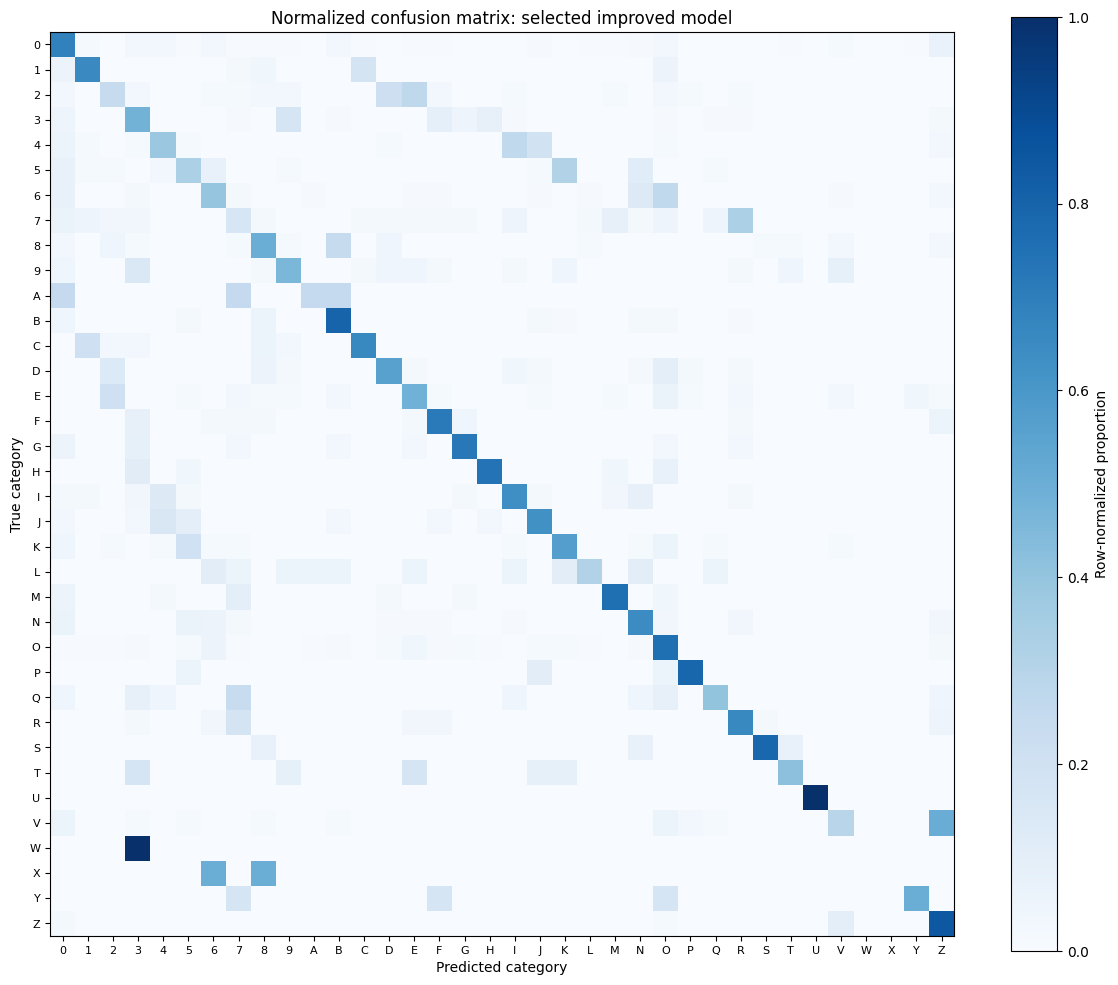
\includegraphics[width=\linewidth]{improved_confusion_matrix}
\caption{Confusion matrix for the improved model, showing strong diagonal performance for distinctive categories and cross-confusion among numeric procedure codes.}
\label{fig:confusion}
\end{figure}

Inspecting the top-weighted TF-IDF features per category confirms the model learns medically meaningful character patterns: \texttt{O}~(pregnancy) captures \textit{``parto''} and \textit{``embara(zo)''}; \texttt{Z}~(health status) captures \textit{``grup(o)''} and \textit{``sang(uíneo)''}; \texttt{J}~(respiratory) captures \textit{``asma''} and \textit{``bron(quitis)''}; \texttt{I}~(circulatory) captures \textit{``hta''}, \textit{``card(io)''}; \texttt{N}~(genitourinary) captures \textit{``ren(al)''} and \textit{``irc''}. These results provide full interpretability of the classifier's decision process.

\subsection{Final submission}
\label{ssec:final}

The selected model (character n-grams (2,5), $C$=2.0, no class weighting) is retrained on all 11\,584 unique literals, producing a feature matrix of shape $(11\,584 \times 28\,473)$ and a final training accuracy of 0.8596. Predictions for all 36 categories are generated for the 6\,667 leaderboard literals.

\vfill\pagebreak

% ============================================================================
\section{Deep Learning Approach: RoBERTa}
\label{sec:dl}
% ============================================================================

To explore whether dense contextual embeddings can outperform our lexical baselines, we fine-tune \texttt{PlanTL-GOB-ES/roberta-base-biomedical-clinical-es}~\cite{PlanTL2022}, a RoBERTa model pre-trained on Spanish biomedical and clinical corpora.

\subsection{Architecture}
\label{ssec:architecture}

The classification model consists of the pre-trained RoBERTa encoder followed by mean pooling over non-padding token embeddings, a dropout layer ($p=0.1$), and a linear classification head mapping to 36 categories. Unlike the TF-IDF approach, preprocessing is minimal (whitespace normalisation only) to preserve casing, accents, and punctuation that carry semantic value for the language model.

\subsection{Training setup}
\label{ssec:training}

Training uses AdamW optimisation ($\text{lr}=2\times10^{-5}$, weight decay $=0.01$), cross-entropy loss, batch size 128, and early stopping with patience~10. The full training set (13\,700 rows) is split 80/20 for training and validation.

\subsection{Preliminary status}
\label{ssec:dl_status}

\textit{This experiment is currently in progress.} The training pipeline is fully implemented but has not yet completed due to computational requirements. Initial runs encountered a tokeniser compatibility issue that has been identified and fixed. Full results, including validation accuracy and comparison with the TF-IDF baselines, will be reported upon completion.

% ============================================================================
\section{Conclusions}
\label{sec:conclusions}
% ============================================================================

This work demonstrates a principled, iterative approach to automated ICD-10 code category prediction from short Spanish clinical literals. Key findings include:

\begin{enumerate}
\item \textbf{Data understanding is essential.} The EDA revealed that normalisation doubles the effective training coverage (27\% $\to$ 62\% overlap), that ICD descriptions cannot serve as a lookup table (Jaccard $< 0.2$), and that inherent ambiguity (1\,486 multi-category literals) sets a ceiling on achievable accuracy.

\item \textbf{TF-IDF remains competitive.} A carefully tuned character n-gram TF-IDF + Linear SVM pipeline achieves 60.3\% validation accuracy --- a +3.3 percentage point improvement over the baseline --- while remaining fast, interpretable, and fully explainable.

\item \textbf{Principled tuning outperforms capacity increases.} The best model uses \textit{fewer} features per n-gram (2--5 vs.\ 3--6) and a simpler class weighting scheme. Higher-capacity models (word+char union) overfit without improving generalisation.

\item \textbf{ICD knowledge augmentation shows promise.} Preliminary experiments with description augmentation suggest further gains ($\sim$0.619 accuracy), pending cross-validation.

\item \textbf{Deep learning exploration.} Fine-tuning a Spanish biomedical RoBERTa model is underway. Whether dense contextual representations can overcome the extreme brevity of clinical literals remains an open question.
\end{enumerate}

The complete codebase, including shared preprocessing and evaluation modules, is structured for reproducibility and consistency across all experimental notebooks.

% References
% -------------------------------------------------------------------------
\bibliographystyle{IEEEbib}
\bibliography{refs}

\end{document}
